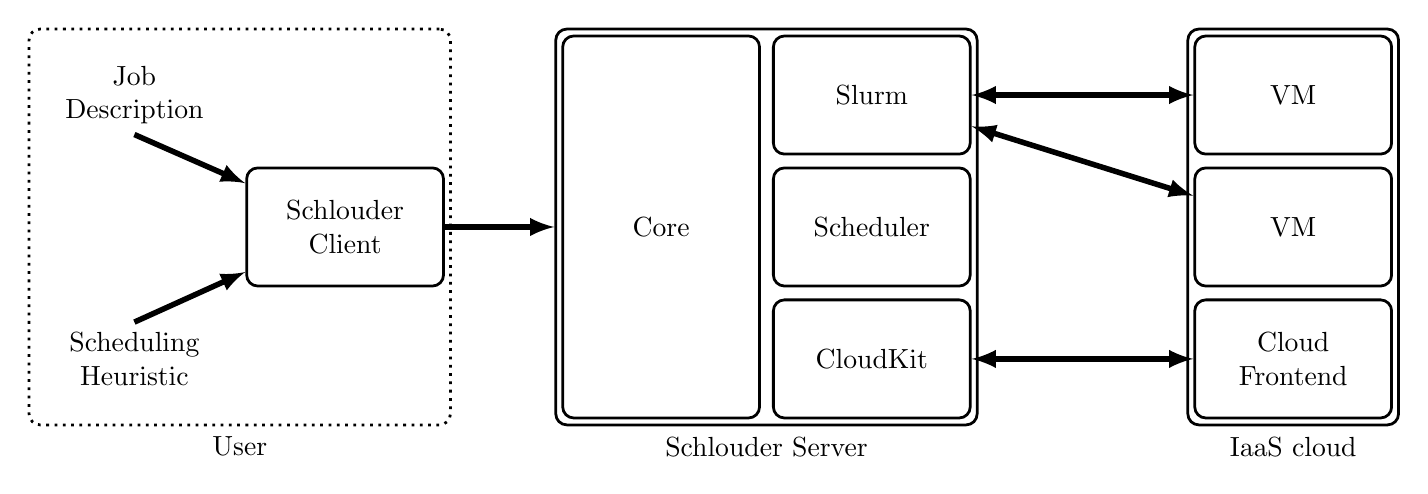
\begin{tikzpicture}[x=25mm+5pt,y=15mm+5pt,
every node/.style={%
line width=1pt,
draw,
rounded corners,
anchor=center,
},
input/.style={draw=none,align=center},
arrw/.style={latex-latex,line width=2pt},
arw/.style={-latex,line width=2pt}
]
\node[minimum height=15mm,minimum width=25mm,align=center]at(-1.5,1)(sc){Schlouder\\Client};
\node[input]at(-2.5,2)(JD){Job\\Description};
\node[input]at(-2.5,0)(SH){Scheduling\\Heuristic};
\node[minimum height=45mm+15pt,minimum width=50mm+10pt,label={[]south:User},dotted]at(-2,1){};
\node[minimum height=45mm+10pt,minimum width=25mm]at(0,1){Core};
\node[minimum height=15mm,minimum width=25mm]at(1,0)(ck){CloudKit};
\node[minimum height=15mm,minimum width=25mm]at(1,1)(schd){Scheduler};
\node[minimum height=15mm,minimum width=25mm]at(1,2)(slrm){Slurm};
\node[minimum height=45mm+15pt,minimum width=50mm+10pt,label={[]south:Schlouder Server}]at(0.5,1)(ss){};
\node[minimum height=15mm,minimum width=25mm,align=center]at(3,0)(cc){Cloud\\Frontend};
\node[minimum height=15mm,minimum width=25mm]at(3,1)(vm1){VM};
\node[minimum height=15mm,minimum width=25mm]at(3,2)(vm2){VM};
\node[minimum height=45mm+15pt,minimum width=25mm+5pt,label={[]south:IaaS cloud}]at(3,1){};
\draw[arrw](ck)--(cc);
\draw[arrw](slrm)--(vm1);
\draw[arrw](slrm)--(vm2);
\draw[arw](JD.270)--(sc);
\draw[arw](SH.90)--(sc);
\draw[arw](sc)--(ss);
\end{tikzpicture}
